\documentclass[border=10pt]{standalone}

\usepackage{tikz}
\usepackage{tikzsymbols}
\usetikzlibrary{calc,patterns,shapes.geometric}

\def\centerarc[#1](#2)(#3:#4:#5){\draw[#1] ($(#2)+({#5*cos(#3)},{#5*sin(#3)})$) arc (#3:#4:#5);}

\begin{document}
	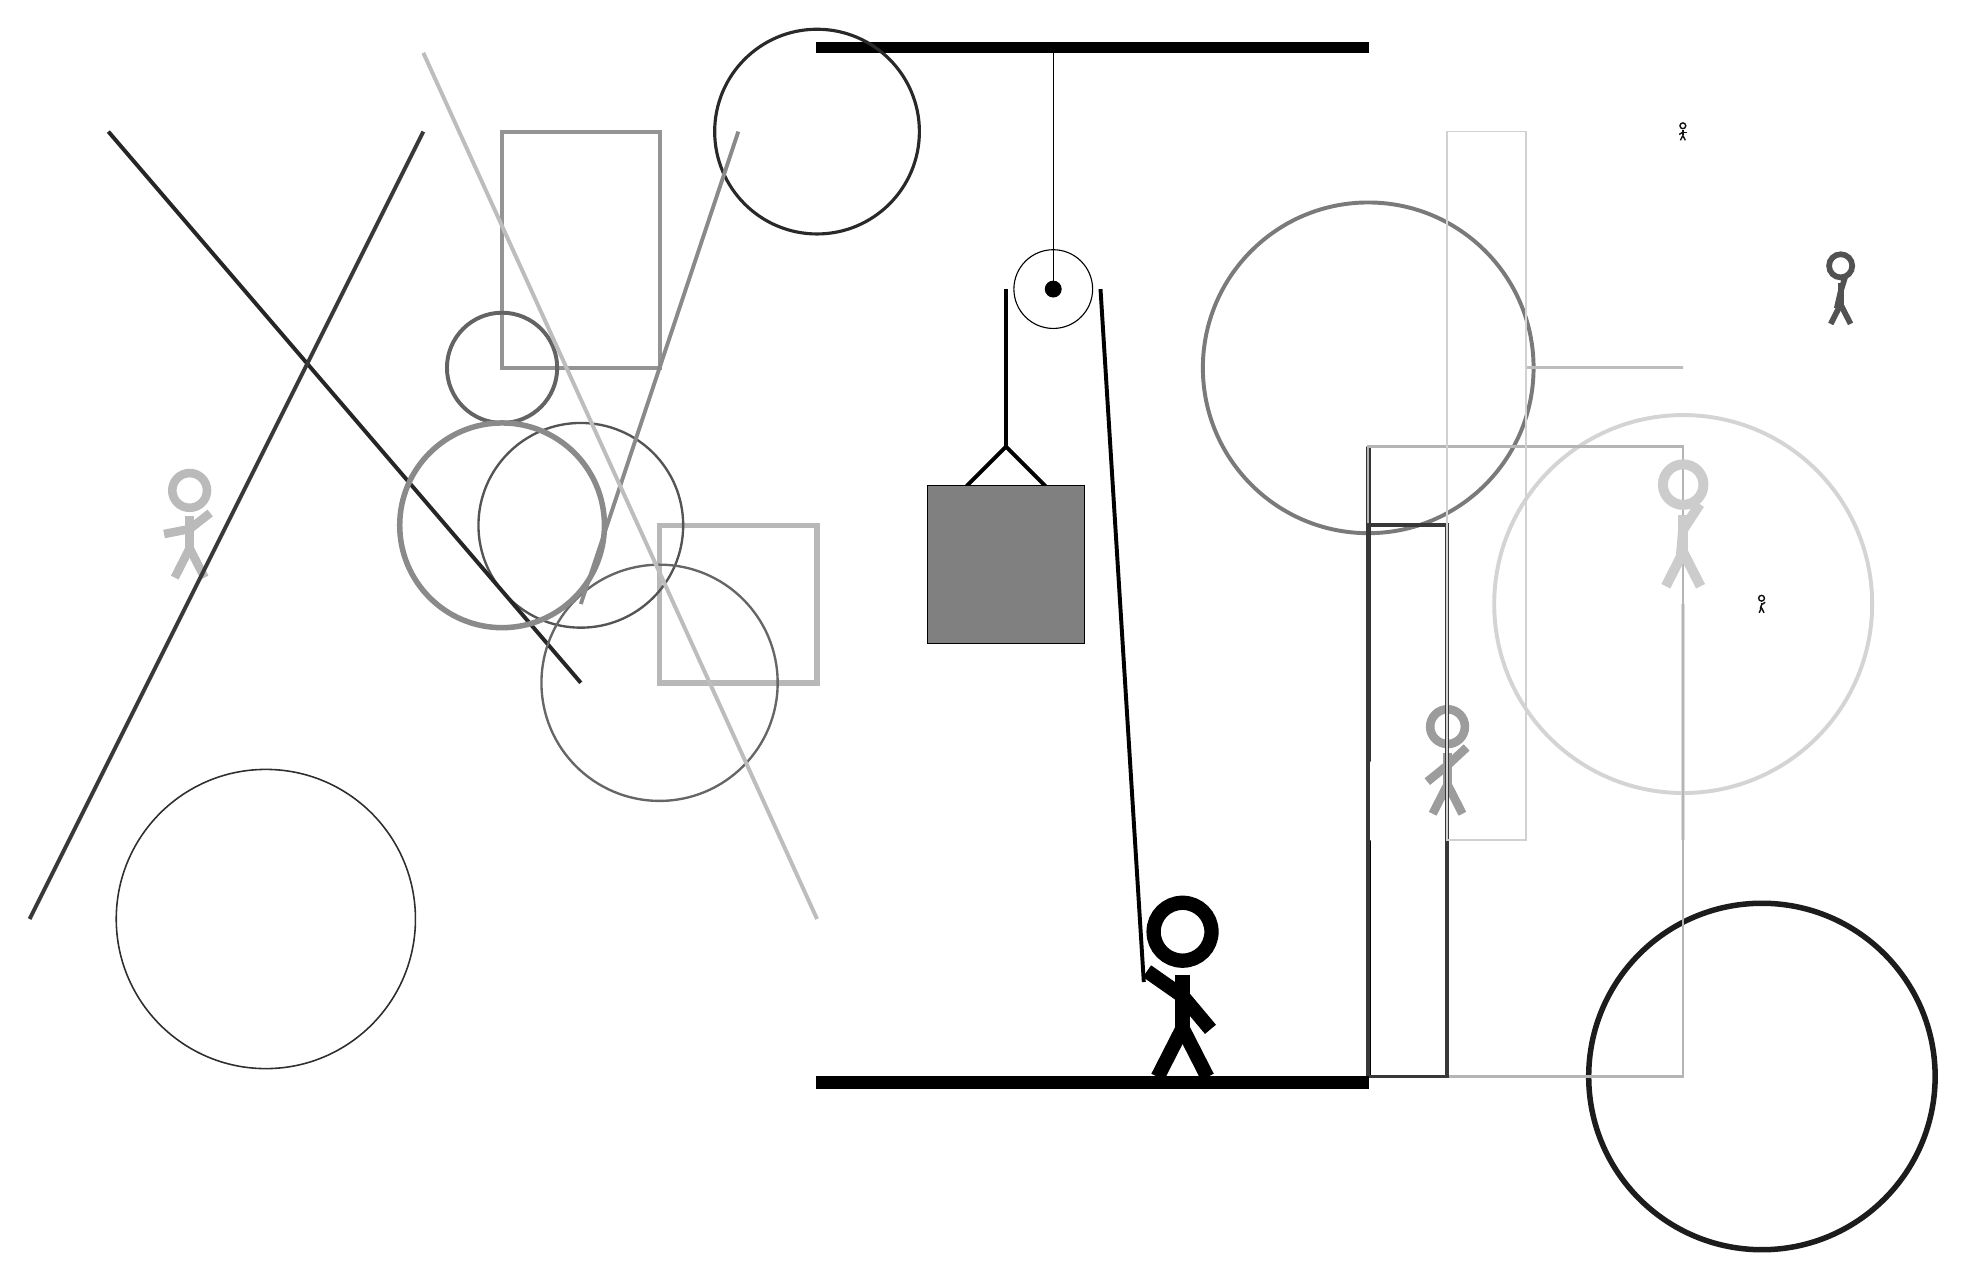
\begin{tikzpicture}
		%%%%% START %%%%%
		
		\draw[fill=black] (-2, 10) rectangle (5, 10.125);
		
		\draw (1, 7) circle (0.5);
		\draw[fill=black] (1, 7) circle (0.1);
		\draw (1, 10) -- (1, 7);
		
		\node[line width=0.4mm, color=black!39] at (6, 1) {\Strichmaxerl[6][39][43]};
		
		\draw[line width=0.5mm, color=black!42] (-4, 6) rectangle (-6, 9);
		\draw [line width=0.7mm, color=black!89](10, -3) circle (2.2);
		\draw [line width=0.5mm, color=black!52](5, 6) circle (2.1);
		\node[line width=0.3mm, color=black!92] at (9, 9) {\Strichmaxerl[1][31][0]};
		\node[line width=0.3mm, color=black!68] at (11, 7) {\Strichmaxerl[4][77][73]};
		
		\draw[line width=0.7mm, color=black!28] (-4, 4) rectangle (-2, 2);
		\draw[line width=0.5mm, color=black!14](9, 0) -- (9, 3);
		\node[line width=0.7mm, color=black!27] at (-10, 4) {\Strichmaxerl[6][11][38]};
		
		\draw[line width=0.6mm, color=black!80] (5, 1) rectangle (5, 5);
		
		\draw [line width=0.3mm, color=black!67](-5, 4) circle (1.3);
		
		\draw [line width=0.5mm, color=black!17](9, 3) circle (2.4);
		\draw [line width=0.4mm, color=black!84](-2, 9) circle (1.3);
		\draw[line width=0.5mm, color=black!85](-5, 2) -- (-11, 9);
		\draw[line width=0.5mm, color=black!78](-7, 9) -- (-12, -1);
		\draw [line width=0.5mm, color=black!61](-6, 6) circle (0.7);
		
		\draw[line width=0.4mm, color=black!26] (7, 6) rectangle (9, 6);
		\draw [line width=0.3mm, color=black!60](-4, 2) circle (1.5);
		\draw[line width=0.5mm, color=black!46](-3, 9) -- (-5, 3);
		\draw[line width=0.3mm, color=black!29] (5, 5) rectangle (9, -3);
		\draw [line width=0.7mm, color=black!46](-6, 4) circle (1.3);
		\draw[line width=0.6mm, color=black!98] (5, 0) rectangle (5, -3);
		\draw [line width=0.2mm, color=black!82](-9, -1) circle (1.9);
		\draw[line width=0.5mm, color=black!78] (5, -3) rectangle (6, 4);
		\node[line width=0.2mm, color=black!93] at (10, 3) {\Strichmaxerl[1][72][33]};
		\draw[line width=0.5mm, color=black!26](-7, 10) -- (-2, -1);
		
		\draw[line width=0.2mm, color=black!18] (7, 9) rectangle (6, 0);
		\node[line width=0.6mm, color=black!20] at (9, 4) {\Strichmaxerl[7][85][57]};
		
		\draw[line width=0.5mm] (-0.1, 4.5) -- (0.4, 5.0) -- (0.9, 4.5);
		\draw[fill=black!50] (-0.6, 4.5) rectangle (1.4, 2.5);
		
		\draw[line width=0.5mm] (0.4, 7) -- (0.4, 5.0);
		\centerarc[line width=0.5mm](1, 7)(0:180:0.6);
		\draw[line width=0.5mm](1.6, 7) -- (2.15, -1.8);
		
		\node at (2.6, -1.9) {\Strichmaxerl[10][-35][-50]};
		
		\draw[fill=black] (-2, -3) rectangle (5, -3.15);
		
		%%%%% END %%%%%
	\end{tikzpicture}
\end{document}